\documentclass[11pt]{article}

\usepackage[margin=1in]{geometry}
\usepackage{booktabs}
\usepackage{tabularx}
\usepackage{pgfplots}
\usepackage{pgfplotstable}
\usepackage{hyperref}
\usepackage{xcolor}

\pgfplotsset{compat=1.18}
\hypersetup{
  colorlinks=true,
  linkcolor=blue!55!black,
  urlcolor=blue!55!black,
  citecolor=blue!55!black
}

\title{Multilingual RefusalBench-NQ Pilot: Research Direction Analysis}
\author{}
\date{June 2026}

\begin{document}
\maketitle

\begin{abstract}
This short report evaluates a pilot extension of RefusalBench-NQ from English into
Russian, Chinese, Polish, and German. The pilot is useful as a feasibility study:
the evaluation pipeline is internally consistent, and the results show that
translation can change both answer accuracy and refusal behavior. However, the
sample is too small and the translation layer too noisy to support quantitative
claims about multilingual model capability. The main research implication is that
multilingual selective refusal appears worth studying, but it requires a larger,
human-validated benchmark design.
\end{abstract}

\section{Pilot Setup}

The pilot sampled 18 English RefusalBench-NQ test examples: one example for each
combination of six perturbation classes and three intensities. Each example was
expanded to five languages: English, Russian, Chinese, Polish, and German. The
query and context were translated with Amazon Translate, while the refusal labels
and reference answers were preserved from the English source item.

Two Bedrock-hosted models were evaluated: \texttt{meta.llama3-8b-instruct-v1:0}
and \texttt{qwen.qwen3-32b-v1:0}. The run produced 180 model predictions
($90$ examples $\times$ $2$ models). Each model--language slice has only 18
examples: 6 answerable examples and 12 unanswerable examples. The LLM judge was
\texttt{bedrock/us.anthropic.claude-sonnet-4-6}. The output files are complete:
all 180 expected predictions are present, and the aggregate metrics recompute
exactly from the raw CSV.

\section{Headline Results}

Figure~\ref{fig:answer-refusal} shows the two most relevant metric families:
answer accuracy on answerable instances and exact refusal-code accuracy on
unanswerable instances. Because each language slice contains only six answerable
examples and twelve unanswerable examples, a single example changes answer
accuracy by 16.7 percentage points and refusal accuracy by 8.3 percentage points.

\begin{figure}[ht]
\centering
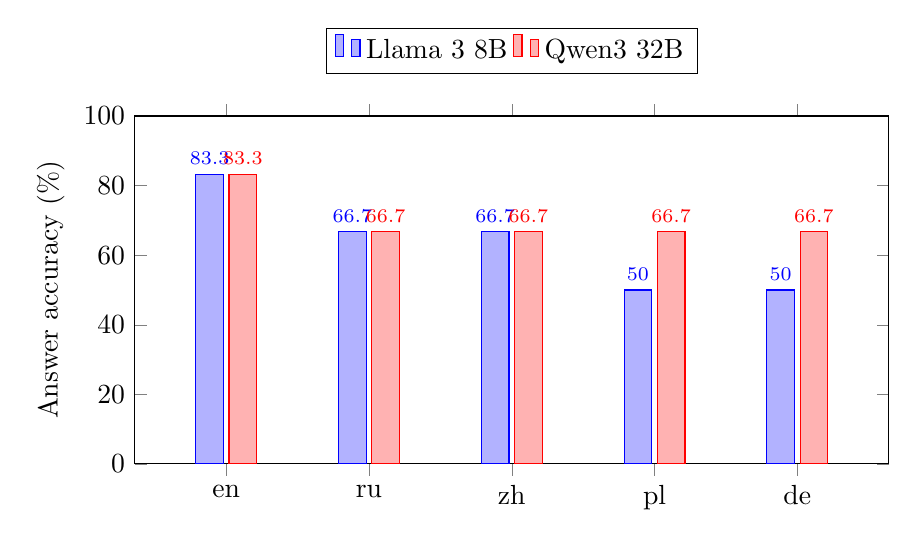
\begin{tikzpicture}
\begin{axis}[
  ybar,
  width=0.92\linewidth,
  height=6.0cm,
  ymin=0,
  ymax=100,
  ylabel={Answer accuracy (\%)},
  symbolic x coords={en,ru,zh,pl,de},
  xtick=data,
  bar width=10pt,
  enlarge x limits=0.16,
  legend style={at={(0.5,1.12)}, anchor=south, legend columns=2},
  nodes near coords,
  nodes near coords align={vertical},
  every node near coord/.append style={font=\scriptsize},
]
\addplot coordinates {(en,83.3) (ru,66.7) (zh,66.7) (pl,50.0) (de,50.0)};
\addplot coordinates {(en,83.3) (ru,66.7) (zh,66.7) (pl,66.7) (de,66.7)};
\legend{Llama 3 8B,Qwen3 32B}
\end{axis}
\end{tikzpicture}

\vspace{0.5cm}

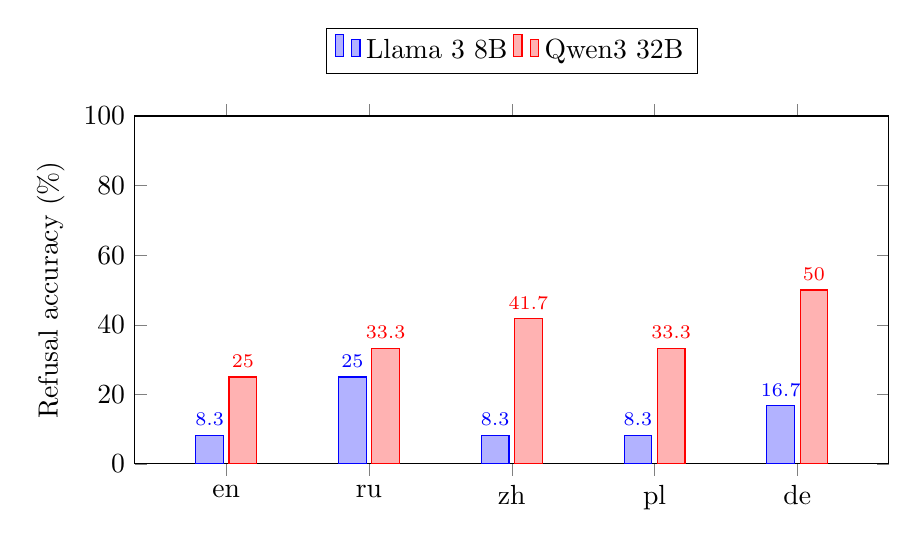
\begin{tikzpicture}
\begin{axis}[
  ybar,
  width=0.92\linewidth,
  height=6.0cm,
  ymin=0,
  ymax=100,
  ylabel={Refusal accuracy (\%)},
  symbolic x coords={en,ru,zh,pl,de},
  xtick=data,
  bar width=10pt,
  enlarge x limits=0.16,
  legend style={at={(0.5,1.12)}, anchor=south, legend columns=2},
  nodes near coords,
  nodes near coords align={vertical},
  every node near coord/.append style={font=\scriptsize},
]
\addplot coordinates {(en,8.3) (ru,25.0) (zh,8.3) (pl,8.3) (de,16.7)};
\addplot coordinates {(en,25.0) (ru,33.3) (zh,41.7) (pl,33.3) (de,50.0)};
\legend{Llama 3 8B,Qwen3 32B}
\end{axis}
\end{tikzpicture}
\caption{Per-language answer accuracy and exact refusal-code accuracy. These
rates are mechanically correct but statistically unstable because each
model--language slice is small.}
\label{fig:answer-refusal}
\end{figure}

The direction of the observed changes differs by model. Llama 3 8B shows lower
answer accuracy outside English, especially in Polish and German, and it false
refuses some translated answerable examples. Qwen3 32B also loses answer accuracy
outside English, but its exact refusal-code accuracy improves in translated
settings, particularly German and Chinese. In paired comparisons against the
English source item, 23 of 72 non-English Llama outcomes and 16 of 72 non-English
Qwen outcomes differ from the corresponding English outcome.

\begin{figure}[ht]
\centering
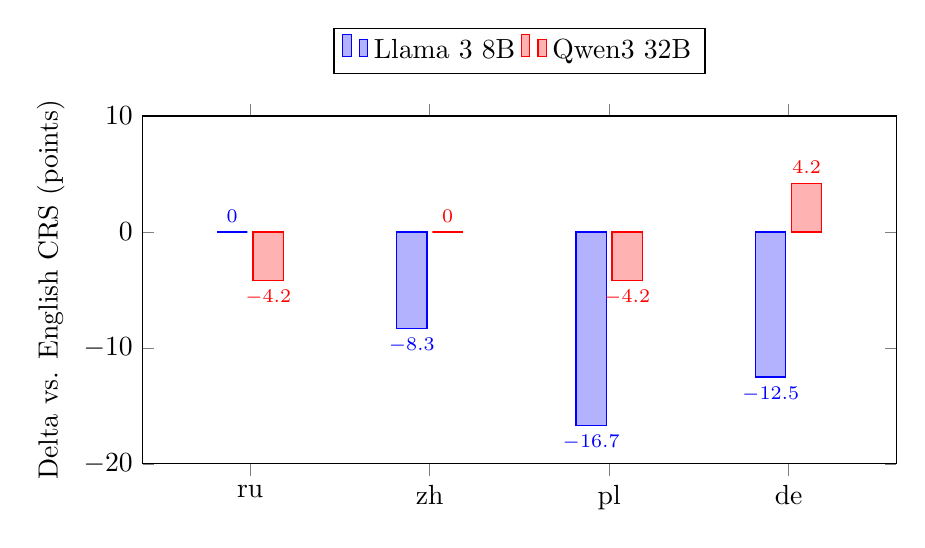
\begin{tikzpicture}
\begin{axis}[
  ybar,
  width=0.92\linewidth,
  height=6.0cm,
  ymin=-20,
  ymax=10,
  ylabel={Delta vs. English CRS (points)},
  symbolic x coords={ru,zh,pl,de},
  xtick=data,
  bar width=11pt,
  enlarge x limits=0.2,
  legend style={at={(0.5,1.12)}, anchor=south, legend columns=2},
  nodes near coords,
  nodes near coords align={vertical},
  every node near coord/.append style={font=\scriptsize},
]
\addplot coordinates {(ru,0.0) (zh,-8.3) (pl,-16.7) (de,-12.5)};
\addplot coordinates {(ru,-4.2) (zh,0.0) (pl,-4.2) (de,4.2)};
\legend{Llama 3 8B,Qwen3 32B}
\end{axis}
\end{tikzpicture}
\caption{Delta in calibrated refusal score (CRS) relative to English. CRS is the
mean of answer accuracy and refusal accuracy. The plot is useful for direction,
not for estimation.}
\label{fig:crs-delta}
\end{figure}

\section{Interpretation}

The pilot suggests that translating RefusalBench-NQ changes the task in ways
that affect both answering and refusing. For Llama 3 8B, translated answerable
items more often become false refusals or lower-quality answers, while refusal
accuracy remains low overall. For Qwen3 32B, translated settings reduce answer
accuracy but sometimes improve exact refusal-code matching. This asymmetry is
important: multilingual effects are not simply a monotonic degradation from
English. Some translations appear to make a refusal problem easier, harder, or
different.

The results should therefore be read as evidence for a research direction rather
than evidence for model ranking. The most plausible research question is not
``which language is harder?'' but rather: \emph{which refusal phenomena survive
translation, which are distorted by translation, and which require
language-specific benchmark construction?}

\section{Translation Quality Issues}

Manual inspection found several examples where machine translation changes the
surface form or likely semantics of the task. These examples are not necessarily
all catastrophic, but they are enough to make the current pilot unsuitable for
strong quantitative claims.

\begin{table}[ht]
\centering
\small
\begin{tabularx}{\linewidth}{@{}p{0.17\linewidth}p{0.27\linewidth}X@{}}
\toprule
Language & Source phenomenon & Observed issue \\
\midrule
German & Ambiguous TV-show context with the channel ``Space'' &
The channel name is translated as \texttt{Weltraum} (outer space), changing an
entity mention into a common noun and potentially altering the ambiguity. \\
\addlinespace
Chinese & ``Traveling Wilburys'' music context &
The band/entity name is semantically translated as a travel phrase rather than
clearly preserved as a named entity, which can blur the entity structure that the
ambiguity perturbation relies on. \\
\addlinespace
Polish & Public-insurance-adjuster answerable item &
``Public adjusters'' becomes an unnatural occupational phrase close to
``public insurance correctors,'' and ``policy holders'' is rendered in a way that
can sound like insurance policies rather than people. \\
\addlinespace
Russian & Insurance-claim answerable item &
The translated context shifts the fee relation: the adjuster appears to
``represent a policyholder receiving a small part'' rather than representing the
policyholder for a percentage fee. \\
\addlinespace
Chinese & Length-ratio heuristic &
All 18 Chinese rows are flagged as length-ratio anomalies. This is partly an
artifact of character count differences, so the warning is useful for triage but
not a reliable translation-failure signal by itself. \\
\bottomrule
\end{tabularx}
\caption{Examples of translation artifacts that can confound multilingual
RefusalBench-NQ evaluation.}
\label{tab:translation-issues}
\end{table}

\section{Limitations}

\paragraph{Small sample.}
The pilot contains one source example per stratum. Per-stratum metrics are
therefore single-example outcomes, and language-level metrics have only six
answerable and twelve unanswerable examples per model.

\paragraph{Machine translation is not benchmark construction.}
The pilot translates English query/context pairs but preserves English-derived
labels and reference answers. This tests translated-input robustness, not a
fully localized multilingual RefusalBench.

\paragraph{English-centric prompting and judging.}
The model instructions, refusal codes, judge rubric, and reference answers are
English-centric. A non-English model answer is judged against English reference
answers, which is usually workable for dates and named entities but may be noisy
for paraphrases, morphology, and culturally specific wording.

\paragraph{Translation can change the perturbation.}
Some RefusalBench perturbations depend on ambiguity, reference, contradiction,
granularity, and named-entity structure. These are precisely the properties that
translation can alter. A translated item may no longer instantiate the same
phenomenon as the English source.

\paragraph{Limited model coverage.}
Only two models were evaluated. The results are not comparable to the full
RefusalBench paper or to larger model suites.

\paragraph{Run reproducibility needs cleanup.}
The final files are complete, but the translation log records an earlier
credential failure. Future runs should write complete run metadata, including
translation command, region, source file checksum, model settings, and judge
version.

\section{Recommended Next Step}

The next study should scale the sample to at least 10 examples per stratum,
manually validate or repair translations, and separate two conditions: (1)
translated-input RefusalBench, where English labels and refusal codes are kept
fixed, and (2) localized RefusalBench, where prompts, labels, examples, and
reference answers are adapted per language. Reporting should include confidence
intervals and paired English-vs-translation analyses rather than only aggregate
language means.

\section{Conclusion}

The pilot pipeline is trustworthy as an engineering check: the dataset,
evaluation output, and aggregate metrics are internally consistent. The research
finding is more cautious: multilingual selective refusal appears sensitive to
translation, but the current pilot cannot separate model behavior from
translation artifacts. The appropriate conclusion is that multilingual
RefusalBench-NQ is a promising research direction, provided the next iteration
uses larger samples and human-validated language-specific data.

\end{document}
